\documentclass{sigchi}\usepackage[]{graphicx}\usepackage[]{color}
%% maxwidth is the original width if it is less than linewidth
%% otherwise use linewidth (to make sure the graphics do not exceed the margin)
\makeatletter
\def\maxwidth{ %
  \ifdim\Gin@nat@width>\linewidth
    \linewidth
  \else
    \Gin@nat@width
  \fi
}
\makeatother

\definecolor{fgcolor}{rgb}{0.345, 0.345, 0.345}
\newcommand{\hlnum}[1]{\textcolor[rgb]{0.686,0.059,0.569}{#1}}%
\newcommand{\hlstr}[1]{\textcolor[rgb]{0.192,0.494,0.8}{#1}}%
\newcommand{\hlcom}[1]{\textcolor[rgb]{0.678,0.584,0.686}{\textit{#1}}}%
\newcommand{\hlopt}[1]{\textcolor[rgb]{0,0,0}{#1}}%
\newcommand{\hlstd}[1]{\textcolor[rgb]{0.345,0.345,0.345}{#1}}%
\newcommand{\hlkwa}[1]{\textcolor[rgb]{0.161,0.373,0.58}{\textbf{#1}}}%
\newcommand{\hlkwb}[1]{\textcolor[rgb]{0.69,0.353,0.396}{#1}}%
\newcommand{\hlkwc}[1]{\textcolor[rgb]{0.333,0.667,0.333}{#1}}%
\newcommand{\hlkwd}[1]{\textcolor[rgb]{0.737,0.353,0.396}{\textbf{#1}}}%

\usepackage{framed}
\makeatletter
\newenvironment{kframe}{%
 \def\at@end@of@kframe{}%
 \ifinner\ifhmode%
  \def\at@end@of@kframe{\end{minipage}}%
  \begin{minipage}{\columnwidth}%
 \fi\fi%
 \def\FrameCommand##1{\hskip\@totalleftmargin \hskip-\fboxsep
 \colorbox{shadecolor}{##1}\hskip-\fboxsep
     % There is no \\@totalrightmargin, so:
     \hskip-\linewidth \hskip-\@totalleftmargin \hskip\columnwidth}%
 \MakeFramed {\advance\hsize-\width
   \@totalleftmargin\z@ \linewidth\hsize
   \@setminipage}}%
 {\par\unskip\endMakeFramed%
 \at@end@of@kframe}
\makeatother

\definecolor{shadecolor}{rgb}{.97, .97, .97}
\definecolor{messagecolor}{rgb}{0, 0, 0}
\definecolor{warningcolor}{rgb}{1, 0, 1}
\definecolor{errorcolor}{rgb}{1, 0, 0}
\newenvironment{knitrout}{}{} % an empty environment to be redefined in TeX

\usepackage{alltt}

% Use this command to override the default ACM copyright statement (e.g. for preprints). 
% Consult the conference website for the camera-ready copyright statement.

%% EXAMPLE BEGIN -- HOW TO OVERRIDE THE DEFAULT COPYRIGHT STRIP -- (July 22, 2013 - Paul Baumann)
\toappear{%$^\ast$ All authors contributed equally. \\
Permission to make digital or hard copies of all or part of this work for personal or classroom use is 	granted without fee provided that copies are not made or distributed for profit or commercial advantage and that copies bear this notice and the full citation on the first page. Copyrights for components of this work owned by others than ACM must be honored. Abstracting with credit is permitted. To copy otherwise, or republish, to post on servers or to redistribute to lists, requires prior specific permission and/or a fee. Request permissions from permissions@acm.org. \\
{\emph{L@S'15}}, March 14--15, 2015, Vancouver, Canada. \\
Copyright \copyright~2015 ACM ISBN/14/04...\$15.00. \\
DOI string from ACM form confirmation}
%% EXAMPLE END -- HOW TO OVERRIDE THE DEFAULT COPYRIGHT STRIP -- (July 22, 2013 - Paul Baumann)


% Arabic page numbers for submission. 
% Remove this line to eliminate page numbers for the camera ready copy
\pagenumbering{arabic}


% Load basic packages
\usepackage{balance}  % to better equalize the last page
\usepackage{graphics} % for EPS, load graphicx instead
\usepackage{times}    % comment if you want LaTeX's default font
\usepackage{url}      % llt: nicely formatted URLs
\usepackage{booktabs}
\usepackage{rotating}

% llt: Define a global style for URLs, rather that the default one
\makeatletter
\def\url@leostyle{%
  \@ifundefined{selectfont}{\def\UrlFont{\sf}}{\def\UrlFont{\small\bf\ttfamily}}}
\makeatother
\urlstyle{leo}


% To make various LaTeX processors do the right thing with page size.
\def\pprw{8.5in}
\def\pprh{11in}
\special{papersize=\pprw,\pprh}
\setlength{\paperwidth}{\pprw}
\setlength{\paperheight}{\pprh}
\setlength{\pdfpagewidth}{\pprw}
\setlength{\pdfpageheight}{\pprh}

% Make sure hyperref comes last of your loaded packages, 
% to give it a fighting chance of not being over-written, 
% since its job is to redefine many LaTeX commands.
\usepackage[pdftex]{hyperref}
\hypersetup{
pdftitle={SIGCHI Conference Proceedings Format},
pdfauthor={LaTeX},
pdfkeywords={SIGCHI, proceedings, archival format},
bookmarksnumbered,
pdfstartview={FitH},
colorlinks,
citecolor=black,
filecolor=black,
linkcolor=black,
urlcolor=black,
breaklinks=true,
}

% create a shortcut to typeset table headings
\newcommand\tabhead[1]{\small\textbf{#1}}


% End of preamble. Here it comes the document.
\IfFileExists{upquote.sty}{\usepackage{upquote}}{}
\begin{document}

\title{Attrition in Massive Open Online Courses: Inequalities, Dropout Reasons, and Psychological Factors}

\numberofauthors{2}
\author{
  \alignauthor Omitted for blind review\\
  \affaddr{Institution}\\
  \affaddr{Address}\\
  \email{Email}\\
%   \alignauthor Ren\'{e} F. Kizilcec$^\ast$\\
%     \affaddr{Department of Communication}\\
%     \affaddr{Stanford University}\\
%     \email{kizilcec@stanford.edu}\\
%   \alignauthor Sherif Halawa$^\ast$\\
%     \affaddr{Department of Electrical Engineering}\\
%     \affaddr{Stanford University}\\
%     \email{halawa@stanford.edu}\\
}

\maketitle

\begin{abstract}
Research on attrition has a long tradition in the field of education. Large-scale open learning environments prompted a shift away from a monolithic notion of success toward a more nuanced treatment that accounts for the diversity in learners' motivation. A systematic analysis of predictors of and reported reasons for attrition in 17 massive open online courses revealed gender and geographic inequalities in persistence and performance (Study 1). Time was a critical obstacle for many learners, but satisfaction was only weakly related to persistence. A follow-up study with online learners who disengaged from the course (Study 2; $N = 756$) found self-ascribed successful learners to report higher levels of goal striving, feelings of social belonging, and growth mindset. Iterative coding of open responses about challenges learners faced while taking the course reiterated the prevalence of having not enough time (reported by 84\%). A low capacity for volitional control was identified as a large contributor to this issue. A better understanding of why learners disengage from MOOCs allows for earlier recognition of impending attrition, which enables targeted interventions to help learners achieve their goals.
\end{abstract}

\keywords{Online learning, persistence, attrition, dropout, disengagement, massive open online courses, MOOC, psychological factors}

\category{H.5.m.}{Information Interfaces and Presentation (e.g. HCI)}{Miscellaneous}
\category{K.3.1.}{Computers and Education}{Computer Uses in Education}



\section{Introduction}

Educational environments have become increasingly diverse. Traditional schools and universities have a characteristically rigid structure, including instructor-defined---even nationally agreed---syllabi, fixed time schedules, entry requirements, and material costs to enter and exit. Novel institutional structures have been developed to overcome particular constraints. Community colleges, for instance, were created in an attempt to democratize education by offering instruction at a lower cost, with lower admission criteria, and with more flexible schedules to accommodate those who cannot afford to be full-time students \cite{goldrick2010challenges}. Distance learning programs intended to deliver education in remote parts of the world and for people who simply could not attend in-person classes. Course materials, including assessments, were delivered through mail (correspondence education), radio, television, and eventually the Internet, thereby addressing geographical and time related constraints of traditional instruction \cite{moore1996distance}.

The latest generation of online learning environments, characterized by massive open online courses (MOOCs), has pushed the boundary on the scale of education \cite{waldrop2013campus}. By design, MOOCs provide course materials to millions of people worldwide. This scale could be achieved by pre-recording lectures, designing assessments that can be graded automatically, and by leveraging the momentum of the number of people involved (e.g., to facilitate peer learning or peer grading \cite{kulkarni2013peer,cambre2014talkabout}). Maybe by virtue of their large scale, their prominent instructors, or their adherence to contemporary interface designs, MOOCs rapidly became an online media phenomenon. People would sign up weeks in advance of the course launch date, many of whom would never even enter the course site. And among those who enroll and enter the site, a large proportion tends to only ``sample'' some content and leave again \cite{kizilcec2013deconstructing}. Many of the prototypical behaviors observed in MOOCs \cite{kizilcec2013deconstructing,breslow2013studying} resemble those on online media platforms. This trend has also been reflected in the diversity of MOOC learners' motivations for enrolling \cite{kizilcec2015motivation}.

Shortly after the first wave of courses had finished, extensive media coverage led to MOOCs becoming associated with high attrition rates \cite{lewin2013after,parr2013mooc,guthrie2013moocs}. Early MOOC research cautioned against dichotomizing learners into successes and failures based on course completion \cite{kizilcec2013deconstructing,rivard2013measuring}. Instead, more nuanced categorizations based on learner behavior \cite{kizilcec2013deconstructing,clow2013moocs}, motivations \cite{kizilcec2015motivation}, or intentions \cite{wilkowski2014student} have been suggested. Ultimately, perspectives on persistence and attrition in MOOCs depend on how MOOCs have been conceptualized. Kizilcec and Schneider \citeyear{kizilcec2015motivation} proposed that MOOCs have bridged two different worlds: one is governed by the user-centric norms of online media, where everyone is encouraged to be as active as they wish; the other adheres to the ``grammar of schooling'', which presupposes instructor-defined goals that students strive to achieve \cite{tyack1994grammar}. Viewing MOOC participation as bridging these two worlds undoubtedly adds a layer of complexity to interpretations of attrition. The present work extends the empirical base of research on attrition to inform the theoretical discourse and pave the path for novel practices.

This paper presents a systematic investigation of attrition in MOOCs, based on self-report and behavioral data collected from 66,076 online learners in 18 courses overall. A better understanding of why learners disengage from MOOCs allows for earlier recognition of impending attrition, which enables targeted interventions to help learners achieve their learning goals. We begin by briefly reviewing the large literature on attrition in educational environments with a focus on important developments in understanding its causes. Building on this foundation of prior work, Study 1 offers insights into reasons for disengaging from MOOCs and explores relationships with prior behavior and reported intentions. In Study 2, to develop a deeper understanding of MOOC attrition, we invited around 6,500 learners who were predicted to have disengaged from a MOOC to provide feedback. Their open response answers about what challenges they faced while taking the MOOC were iteratively coded. We investigated the role of volitional control for learners who report having not enough time, and examine goal striving, social belonging, and growth mindset in relation to being successful in a MOOC.

\begin{table*}[th]
\label{tab:s1sum}
\caption{Summary statistics of learner demographics and behavior in 17 MOOCs}
\small
\center
\begin{tabular}{llccccccccccc}
% & & & & & & & & $>$ 30\% & $>$ 50\% & $>$ 80\% & Self-Rep. \\
% & Topic Area & Enrollment & Course survey & Feedback survey & Female & Age & Education & videos & videos & videos & Dropout \\
\toprule
 &            &          & \multicolumn{3}{c}{Survey Responses} & & & & & \multicolumn{3}{c}{Videos Watched} \\
 \cmidrule(r){4-6} \cmidrule(r){11-13}
 & Topic Area & Enrolled & Initial & Feedback & Both & Female & Age$^1$   & Education$^2$ & Dropout$^3$ & $>$ 30\% & $>$ 50\% & $>$ 80\% \\
\midrule
C1 & Business & 61,096   & 9,943  & 2,367    & 1,282    & 42\%   & 39 (30,49) & n.a.       & 10\% & 39\% & 20\% & 7\% \\
C2 & Business & 41,081   & 6,544  & 883      & 630      & 40\%   & 39 (30,49) & 97\%       & 9\%  & 32\% & 13\% & 2\% \\
C3 & CS       & 27,104   & 6,104 & 2,854     & 2,116    & 35\%   & 30 (22,41) & 74\%       & 2\%  & 67\% & 40\% & 7\% \\
C4 & CS       & 56,154   & 3,406 & 1,123     & 352      & 11\%   & 33 (27,42) & 91\%       & 21\% & 34\% & 16\% & 11\% \\
C5 & CS       & 57,636   & 5738  & 402       & 342      & 17\%   & 33 (26,43) & 91\%       & 14\% & 66\% & 55\% & 28\% \\
C6 & Engineering & 16,220 & 2,540 & 269      & 182      & 13\%   & 33 (27,45) & 92\%       & 15\% & 62\% & 49\% & 17\% \\
C7 & Enginerring & 7,178 & 1,312 & 202       & 167      & 12\%   & 27 (22,39) & 85\%       & 7\%  & 51\% & 18\% & 2\% \\
C8 & Humanities & 7,634 & 3,631  & 152       & 127      & 92\%   & 33 (26,45) & 93\%       & 7\%  & 45\% & 11\% & 0\% \\
C9 & Humanities & 6,475 & 3,315  & 326       & 262      & 90\%   & 32 (27,47) & 91\%       & 16\% & 69\% & 50\% & 17\% \\
C10 & Humanities & 9,903 & 4,227 & 1,570     & 1,066    & 52\%   & 39 (29,52) & 89\%       & 3\%  & 84\% & 74\% & 21\% \\
C11 & Humanities & 630 & 167     & 80        & 40       & 50\%   & 30 (27,40) & 97\%       & 16\% & 74\% & 55\% & 16\% \\
C12 & Math \& Stats & 49,317 & 3,090 & 862   & 510      & 33\%   & 41 (29,55) & 88\%       & 31\% & 27\% & 10\% & 1\% \\
C13 & Math \& Stats & 32,006 & 26,142 & 5,336 & 4,096   & 58\%   & 28 (16,46) & n.a.       & 4\%  & 69\% & 38\% & 8\% \\
C14 & Math \& Stats & 16,857 & 2,892 & 363   & 282      & 9\%    & 31 (26,38) & 99\%       & 14\% & 61\% & 45\% & 25\% \\
C15 & Math \& Stats & 37,017 & 11,629 & 1,854 & 1,521   & 20\%   & 35 (29,45) & 98\%       & 8\%  & 78\% & 67\% & 34\% \\
C16 & Math \& Stats & 27,236 & 2,711 & 637   & 610      & 82\%   & 43 (34,51) & n.a.       & 1\%  & 64\% & 36\% & 5\% \\
C17 & Math \& Stats & 13,132 & 3,629 & 843   & 626      & n.a.   & n.a.       & n.a.       & 5\%  & 70\% & 54\% & 14\% \\
\bottomrule
\multicolumn{13}{l}{$^1$ mean (upper, lower quartile)  $^2$ bachelor's or higher degree  $^3$ self-reported in the feedback survey}
\end{tabular}
\end{table*}


\section{Related Work}

Research and theorizing on attrition in education has a rich history. This review is intended to serve as a foundation to build on with the current research. We therefore simultaneously develop research questions and hypotheses to investigate and test in the current work. The focus of this brief review is on how ways of thinking about attrition have developed over the last decades. 

\subsection{In-person Education}

The majority of early work on attrition centered around theoretical models of students' decision to persist or dropout of a traditional higher education setting. The literature on attrition in higher education is largely concerned with students disengaging from a course of study rather than a single course. An early model suggested that students' presistence is largely driven by their prior behavior, attitudes, and norms \cite{fishbein1975belief}. The psychological processes involved in turning an intent to learn into the decision to persist were thought to be mediated by volition, i.e., the extent to which the student engages in goal-direct behaviors in the face of distraction \cite{corno1993role}. Hence, motivation alone is necessary but not sufficient for persistence. Students may fail to sustain efforts in the absence of strong self-regulatory skills.

\begin{description}
  \item[H1] Successful MOOC learners exhibit higher levels of goal striving than unsuccessful ones.
\end{description}

The next generation of psychological models, which were highly influential in the literature, emphasized the critical role of students' ``fit'' in the institution. Tinto's \citeyear{tinto1975dropout} student integration model posited that college students' decision to persist is a function of prior experiences and individual students' characteristics, and experiences during college. While prior experiences and characteristics are fixed, schools can influence the college experience, including the degree of social and academic integration. Tinto operationalized academic and social integration by GPA scores and the frequency of positive interactions with peers and instructors, respectively. This resonates with recent work highlighting the critical role of students' feelings of social belonging in achievement-oriented environments \cite{walton2007question}. 

\begin{description}
  \item[RQ1] How do prior learner characteristics (demographics, geographic location, intentions, and prior experience) influence learners' likelihood of disengaging from a MOOC?
  \item[H2] Successful MOOC learners exhibit a greater sense of social belonging than unsuccessful ones.
\end{description}

Tinto's work, which specifically targets traditional college students, prompted universities to be proactive in establishing environments that support student integration. Research on attrition in community college settings reiterates the importance of academic and social integration, but points out that non-persistence could indicate success depending on students' intent---students may leave after accomplishing their goal \cite{bers1991persistence}. Nevertheless, a brief psychological intervention that taught community college students an incremental theory of intelligence (i.e., instilling a growth mindset) was found to halve attrition rates and increase academic achievement \cite{paunesku2012brief}. The results highlight the powerful influence of mindset and caution against overinterpreting non-persistence as an indicator of goal achievement.

\begin{description}
  \item[RQ2a] What proportion of learners who disengaged were satisfied with their achievements in the course?
  \item[RQ2b] How does learners' behavior in the MOOC vary by their level of satisfaction?
  \item[H3] Successful MOOC learners have a more fluid conception of intelligence (i.e., more of a growth than fixed mindset) than unsuccessful ones.
\end{description}

\subsection{Distance Education and e-Learning}

Distance education, in contrast to traditional in-person education, attracts a different student demographic and typically provides fewer opportunities for social integration. However, students in distance learning programs tend to lead social lives outside of school, maybe working part-time and living with their partner. Building on Tinto's model, Bean and Metzner \citeyear{bean1985conceptual} proposed a conceptual model of persistence that would be more applicable to nontraditional students. Persistence is thought to be a function of background characteristics (e.g., demographics), academic and environmental variables (e.g., study habits, financial resources, work and family obligations), and academic and psychological outcomes (e.g., GPA, satisfaction). The significant change from Tinto's orginal model was the inclusion of environmental variables to account for the added complexity of nontraditional students' lives (see \cite{kember1989longitudinal}, for another adaptation of Tinto's model for distance education).

Rovai \citeyear{rovai2003search}, combining Tinto's and Bean and Metzner's models with factors specific to online learning and pedagogical styles, proposed a composite persistence model specifically for students in online distance education programs. Among other novel factors, Rovai's model acknowledges the critical role of computer literacy in online learning. And yet, while the theoretical models become more developed, they became harder to apply to real-world settings, and hence, the empirical evidence to support them remained sparse. An exploratory study of reasons for attrition suggested the following eight constructs, based on over 1,000 online education students: academic and technical skills, learner motivation, time and support for studies, cost and access to the Internet, and technical problems \cite{muilenburg2005student}. An analysis of student behavior on an online education platform showed that 31\% of variation in achievement could be accounted for by a small set of participation measures \cite{morris2005tracking}.

\subsection{MOOCs}

A survey of over one hundred learners who dropped out of a MOOC showed that the majority indicated having too little time due to work responsibilities, not enough social support inside and outside of the course, and insufficient academic and technical support from the course \cite{gutl2014attrition}. A qualitative analysis of public records, especially forum posts, from 42 MOOCs suggested the following reasons for attrition: lack of time, learner motivation, feelings of isolation, lack of interactivity, insufficient prior knowledge or skills, and hidden costs \cite{khalil2014moocs}. A survival analysis of close to 800 learners who had posted on a MOOC discussion forum suggested that the likelihood of dropout was lower for those who i. actively participated in the first week of the course; ii. served as an authority figure in the community on the forum, and iii. did not engage in a particular subcommunity on the forum \cite{yang2013turn}. In addition, a number of machine learning approaches yielded promising results for early dropout prediction (e.g. \cite{taylor2014likely,halawa2014dropout}), but fell short of offering insights into why a given learner would leave the course.

\begin{description}
\item[RQ3a] What reasons do learners report for disengaging from a MOOC?
\item[RQ3b] How do reasons for disengaging vary across prior learner characteristics (cf. RQ1)?
\end{description}  

\section{Study 1: Attrition \& Satisfaction}

The present study extends the existing literature on persistence with a representative quantitative treatment of attrition in MOOCs. We address the research questions developed in the previous section with a combination of self-report and behavioral data from seventeen diverse MOOCs. Going beyond specific research questions, this observational analysis is intended to inform our understanding of attrition in MOOCs to better support learners in these environments. This can be achieved through general changes, for instance, to the course format; or by targeted interventions that support a particular group of learners, such as those who exhibit low levels of goal striving (cf. Study 2).

\subsection{Methods}

Seventeen MOOCs on topics in a variety of disciplines were selected for investigation (see Table \ref{tab:s1sum}). For each course, we merged data from the initial course survey (distributed in the first weeks of the course), the feedback surveys (distributed in the last weeks of the course), and behavioral data collected in the learning environment. 
% Only those learners who completed the feedback survey were included in the analyses (some did not complete the initial course survey). 
On the initial course surveys, learners reported their gender, age, education, prior experience with the topic and MOOCs, enrollment intentions (on the OLEI scale \cite{kizilcec2015motivation}), and how many hours per week they intend to spend on the course. On the feedback survey, learners reported their satisfaction with the course (6-item index, $M=5.29, SD=0.94, \alpha=.82$), and whether they `stopped participating in the course before it ended' or `remained active until the end'. Those who indicated that they stopped participating also reported `what influenced their decision to stop participating' using a grid of 14 binary-choice items (see reasons in Figure \ref{fig:s1reason}).\footnote{Instead of a select-all-that-apply question, we opted for binary-choice items to encourage learners to consider each reason in turn. The response options were ``Did influence my decision to stop" and ``Did NOT influence my decision to stop," which should reduce acquiescence bias relative to yes/no or true/false scales.} Geographic location was determined by IP address.

Table \ref{tab:s1sum} provides summary statistics for enrollment, survey response rates, demographics, self-reported dropout, and a subset of behavioral indicators for each course. Behavioral indicators were chosen to represent course milestones: watching over 30\%, 50\%, 80\% of lecture videos, attempting over 30\%, 50\%, 80\% of assessments, and achieving a grade above the 60$^\text{th}$, 80$^\text{th}$ percentile. A regression analysis predicting course milestones and performance was performed based on a subset of learners who completed the initial course survey in the 17 MOOCs in our dataset. Out of the 63,620 learners who started the survey, we selected those with up to three missing values in the dataset, yielding a sample of $N=44,382$. Missing values were multiply imputed based on other survey responses and pooled estimates are reported, which account for the added uncertainty.\footnote{The $R$ mice package was used to perform multiple imputation and subsequent pooled analyses.}
% The data illustrated in Figure \ref{fig:s1reason} reflect the proportions of learners who selected each reason relative to all learners who reportedly stopped participating in each course.
% The correlation matrixes in Tables \ref{tab:s1reascor} and \ref{tab:s1cor2} are a linear combination of correlation matrixes for each course, assigning equal weight to all courses to discount for considerable variation in sample sizes.
% Information about age, gender, and education level were only available for learners who completed the initial course survey.
% We also computed the fraction of videos in the course each learner had watched to relate self-report measures to learner behavior
 
\subsection{Results}

We address the research questions developed in the previous section in three parts: first, a regression analysis of differential attrition and performance ($RQ1$); second, a comparison of satisfaction levels across subsets of learners ($RQ2ab$), and third, a descriptive analysis of reported reasons for disengaging from the course ($RQ3ab$).

\subsubsection{Individual Differences in Attrition}

We fit logistic mixed-effects (hierarchical) models to a number of binary persistence and performance metrics to estimate individual differences in prior learner characteristics, including demographic and geographic features. Correlations between predictors were low enough to allow for simple interpretation of coefficients. Fourteen MOOCs in the dataset were modeled as a random effect, in order to generalize to the population of similar MOOCs.\footnote{The required data for 3 of the 17 MOOCs could not be obtained in time for submission due to technical issues.} Figure \ref{fig:s1coefs} illustrates regression coefficients with 95\% confidence intervals from each model. The coefficients represent changes from a baseline (intercept) population: male learners in North America, with an average age, who had not earned a bachelor's degree and had no prior experience with the topic or taken other MOOCs, not intending to complete the course, and prepared to spend only up to two hours per week on the course.

A number of significant and substantial individual differences emerged, some indicative of potential inequalities: Women were 10 to 15\% less likely than men to persist with lectures and assessments. Women are also less likely to score a grade above the 60$^\text{th}$ percentile than men. Learners in Africa, Asia, and South America were 20 to 50\% less likely to persist in video watching and tended to achieve lower grades than learners in North America. In contrast, learners in Europe exhibited 20 to 50\% higher persistence with lectures and assessemnts than learners in North America. While learners in Asia exhibited lower persistence with videos, they were more likely to attempt more assessments than learners from North America. 

Besides gender and geography, the older the learner, the more likely they were to persist in lectures and assessments, but the lower their relative performance. More educated learners, those with a bachelor's or higher degree, were somewhat more likely to start assessments, compared to those with less education, but were less likely to perform highly on them. Not surprisingly, prior experience, intending to learn about all topics in the course, and being prepared to spend more hours in the course were strong predictors of persistance. Learners who took prior MOOCs, however, were less likely to persist, yet achieved higher grades.

\begin{knitrout}
\definecolor{shadecolor}{rgb}{0.969, 0.969, 0.969}\color{fgcolor}\begin{figure*}[ht]

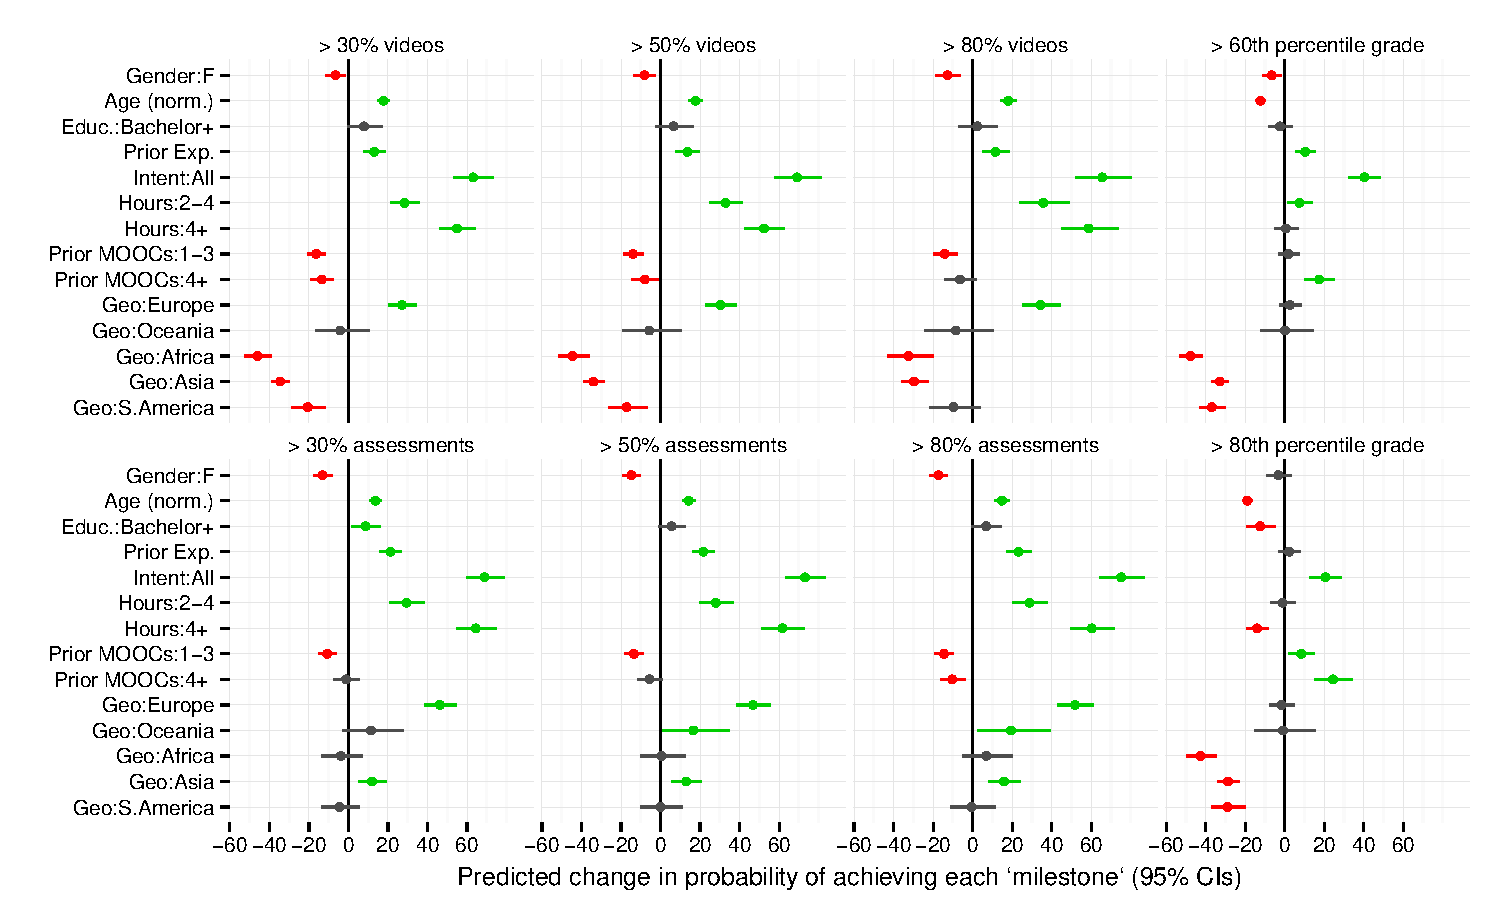
\includegraphics[width=\maxwidth]{figure/s1coefs} \caption[Coefficients of predictors (binary, except for normalized age) from logistic mixed-effects model predicting persistence and performance milestones (prop]{Coefficients of predictors (binary, except for normalized age) from logistic mixed-effects model predicting persistence and performance milestones (prop. videos watched, prop. assessments completed, and grade percentile). The baseline group were male learners in North America of average age who had not earned a bachelor's degree, without prior experience in the topic or other MOOCs, not intending to complete the course, and prepared to spend under two hours per week on it. An estimate of -20 indicates a 20\% lower probability of achieving a milestone.\label{fig:s1coefs}}
\end{figure*}


\end{knitrout}

\subsubsection{Learner Satisfaction}
% RQ2a: What proportion of learners who disengaged were satisfied with their achievements in the course?
% RQ2b: How does learners' behavior in the MOOC vary by their level of satisfaction?

Attrition can be a sign of success if a learner has achieved their personal goal. We therefore investigated to what extent learners were satisfied with their achievements for those who reported to have stopped participating ($RQ2a$) and those who participanted to different degrees ($RQ2b$). To account for differences across courses, we compared satisfaction scores using mixed-effects models.

Learners who reported that they stopped participating were significantly 9\% less satisfied than those who reported not to have stopped ($t_{15140}=18, p<.001$). Moreover, we examined if persistent learners, those who watched more lectures, were also more satisfied. While the the proportion of videos significantly predicted higher satisfaction ($t_{15700}=12, p<.001$), it was a relatively weak effect. Those who watched all videos were only around 3\% more satisfied than those who watched none, based on a linear fit.



% We also examined differences in satisfaction between learners grouped by certain behaviors. First, we classified learners into 4 groups based on the fraction of course videos they viewed. The box plots for the satisfaction scores in each group are shown in figure \ref{fig:study1_satsfaction_by_vid_groups}. The mean satisfaction score increases slightly as the number of videos viewed by the learners increases, with the exception of the scores reported by learners in the 0-25\% group. Possible reasons for this are learners who join only to view a small part of the course or learners who join merely to explore.



\subsubsection{Reasons for Attrition}
% RQ3a: What reasons do learners report for disengaging from a MOOC?
% RQ3b: How do reasons for disengaging vary across prior learner characteristics (cf. RQ1)?

Research question $RQ3a$ about learners' reasons for disengaging from a MOOC is addressed by examining the proportion of learners who selected reasons for attrition from a pre-defined list.\footnote{This researcher-defined list may not have been collectively exhaustive, which is addressed in Study 2.} The distribution of proportions across 17 MOOCs is illustrated in Figure \ref{fig:s1reason} with boxplots. Two reasons related to having too little time stand out because they were reported by about half of the respondents as influencing their decision to stop participating: the reasons were issues keeping up with deadlines, and the course demanding too much time. Other reasons for attrition were less prevalent, though still reported by around 10\% to 25\% of respondents. Notably, just under 20\% of respondents in a typical course (the median proportion) stopped participating because they had learned what they wanted to learn.

To investigate the underlying factor structure of the reported reasons for disengaging, we conducted an exploratory factor analysis. The optimal number of factors was determined by the parallel analysis criterion and corresponding scree plot. The following five factors emerged: first, {\em general time issues} (course requires too much time; can't keep up with deadlines); second, {\em late start} (starting course late); third, {\em  difficulty} (too advanced, exam too difficult); fourth, {\em format and content} (didn't enjoy online format, confusing videos, materials not explained well), and fifth, {\em expectations} (only exploring, learned all I wanted, not what I'm looking for, not challenging, credential not valuable). Only the technical difficulties item failed to load onto any factor.

We expected reasons for disengaging from the course to vary by learner characteristics ($RQ3b$), such as learners' motivations for enrolling in the course. A correlation matrix of learners' enrollment intentions and their subsequent reasons for disengaging revealed a small number of notable associations. Taking the course with friends or colleagues was correlated with disengaging because the course is not challenging enough, the material is too advanced of the learner's background, and the credential is not valuable enough to the learner ($r=.24, .20, .16$, respectively). Not surprisingly, learners who enrolled to experience an online course tended to stop participating because they were only exploring the course ($r=.17$). Learners looking to improve their English tended to experience technical difficulties ($r=.17$), and those who enrolled for personal growth and enrichment tended to struggle to keep up with deadlines ($r=.16$).

\begin{knitrout}
\definecolor{shadecolor}{rgb}{0.969, 0.969, 0.969}\color{fgcolor}\begin{figure*}[ht]

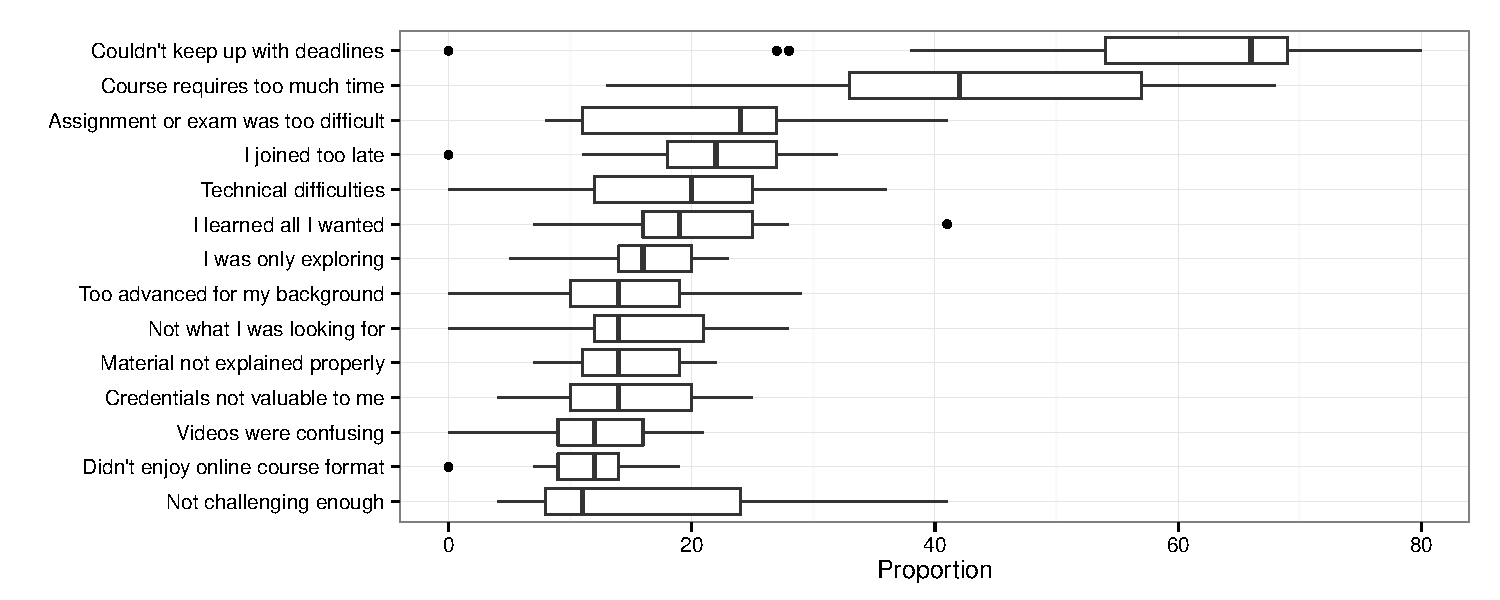
\includegraphics[width=\maxwidth]{figure/s1reason} \caption[Proportion of learners who indicated each reason for attrition across 17 MOOCs]{Proportion of learners who indicated each reason for attrition across 17 MOOCs\label{fig:s1reason}}
\end{figure*}


\end{knitrout}


\subsection{Discussion}

A number of striking findings emerged from the preceeding analyses. We found strong evidence for gender inequalities in attrition and, to some extent, performance. Women were less likely to persist, even when adding a number of other demographic, geographic, and preference indicators to the model, which highlights the robustness of the relationship. The MOOCs in our dataset were on diverse topics, including some on topics in the humanities and business with high rates of participation from women. Besides gender differences, attrition was substantially higher for learners from Africa, Asia, and South America, compared to North America, Oceania, and Europe, in terms of lectures watched. We also identified a large achievement gap in terms of grades between learners from these continents. The current generation of MOOCs is seemingly not immune to inequalities that have pervaded traditional educational settings. It remains unclear, however, to what extent these gaps result from differences in Internet access and language barriers, or potentially, from experiences of psychological threat to learners' identity or sense of social belonging \cite{walton2007question}.

Levels of self-reported satisfaction were generally high and did not vary much by level of persistence, although learners who reportedly disengaged from the course tended to be less satisfied than those who reportedly persisted until the end. Learners' reasons for disengaging from the course clustered into five key factors: general time issues; problems due to starting the course late; course difficulty; issues with the course format or content, and a mismatch or fulfillment of expectations. General time issues were overall the most pronounced. 

Learners may disengage from the course when they become too occupied by higher-priority tasks. Enrolling in a MOOC neither guarantees that a learner can or intends to allocate enough time to go through the course. According to expectancy-value theory, the learner is a rational agent who allocates time to different activities to maximize subjective gain. A low capacity for volitional control \cite{corno2001volitional} could lead learners to misallocate time to lower-priority activities that promise nearer gratification, instead of allocating it to the next highest priority task. This implies that learners' general time issues may be a product of high-priority obligations as well as a result of a low capacity for volitional control.

\section{Study 2: Understanding Attrition}

To gain a better understanding of the attrition patterns identified in Study 1, we designed a smaller, more focused follow-up study. In Study 2, we reached out to learners who were likely to drop out of a course and asked them to provide feedback. To this end, we developed a predictive model to identify disengaging learners and asked them to complete a survey. One goal of this study was to further investigate research question $RQ3a$ about reasons for attrition based on learners' own descriptions of the challenges they faced. Specifically, in Study 1, most learners reported that they disengaged due to a shortage of time. A variety of factors can influence the amount of time learners have at their disposal. Higher priority obligations, such as professional, academic, and personal committments, are presumably large contributors. Another critical factor, especially in the context of MOOCs as largely unguided learning environments, is learners' volitional control to engage in self-regulated learning \cite{corno2001volitional}. For instance, learners' ability to allocate time for the course in the presence of potential distractors of subjectively lower importance than taking the course (e.g., watching TV). We constructed the following hypotheses about the presence of these two factors for learners who report having not enough time:

\begin{description}
  \item[H4a] Learners who report having `not enough time' can be grouped into those with higher priority obligations (professional, academic, and personal) and those with low volitional control.
  \item[H4b] Learners who do not report specific higher-priority obligations tend to exhibit lower volitional control than those who specify particular obligations.
\end{description}  

Another goal of Study 2 was to collect data to test hypotheses $H1, H2,$ and $H3$ on the role of goal striving, social belonging, and growth mindset in the success of MOOC learners. To this end, we included a self-report measure for each construct in the survey that was sent to disengaging learners.

\subsection{Methods}

The particular MOOC under observation was an undergraduate level course on an advanced topic in computer science. It was offered in 2014 through Coursera. There were  20,048 enrolled learners; 10,510 watched at least one video, and 5,912 attempted at least one assignment. The following subsections describe how disengaging learners were identified, which measures were included in the feedback survey, and how open responses were iteratively coded.

\subsubsection{Predicting Disengagement}

We constructed an `early warning' prediction model to flag learners who had disengaged from the course or were about to disengage. The following three criteria were chosen as benchmarks to evaluate the practical and theoretical value of our prediction model.%   In order for our predictions to be useful, we need to observe the following three features of the dropout prediction problem.

\textit{Prediction accuracy}: Prediction recall (fraction of correctly predicted disengaged learners) should be high to deliver the survey to as many disengaged learners as possible. The false positive rate (fraction of active learners who are incorrectly predicted as disengaged) should be low to avoid sending surveys to learners who do not experience challenges in the course.

\textit{Prediction lag}: The period between a learner's last site activity and the time they are flagged as disengaged should be short. A shorter prediction lag improves the likelihood of successfully intervening to help learners resume the course.

\textit{Transferability}: Whether or not a learner disengages from the course cannot be determined before the end of the course. We thus trained the prediction model using data from previous courses. The performance of the prediction model should be good in courses other than those on which it was trained.

The training set was composed of learners' interaction data (predictors) and disengagement states (outcome) from 20 MOOCs. The large number of courses should improve model transferability by favoring features that are strongly predictive across different courses. Five hundred learners from each MOOC were included in the training set ($train$), and 500 other learners from the same MOOCs were selected for the first test set ($test_1$). A second test set of similar size was composed from 20 other MOOCs ($test_2$). Features extracted from the interaction data included different aspects of learners' video, assignment, and forum activity; their pace of viewing videos relative to the course pace, as well as various aspects of engagement time, such as the last time the learner interacted with the course (see omitted for blind review%\cite{halawa2014dropout}
, for additional information on the prediction model).

To control the length of the prediction lag, the model was only provided with learners' activity data until they were absent for 14 consecutive days. In the training phase, if the learner disengaged but the model did not detect it within 14 days of their last activity, the case was counted as a false negative. This construction results in a model with features that all fall within the defined prediction lag period. The model was fit by logistic regression with two-fold learner-level and course-level cross-validation. Table \ref{tab:predAuc} provides information on the prediction performance, measured by the area under the ROC curve (AUC).

\begin{table}[h!]
\caption{Performance of the attrition prediction model}
\label{tab:predAuc}
\small
\center
\begin{tabular}{lccc}
\toprule
 & $train$ & $test_1$ & $test_2$ \\
\midrule
AUC &  0.931 & 0.929 & 0.922  \\
\bottomrule
\end{tabular}
\end{table}

Two of the predictors in the fitted model are highly influential. The first is the number of days since the learner has last been active ($x_{1}$). The likelihood that the learner drops out increases substantially if the learner disengages for 14 days or more. However, the likelihood of such a learner re-engaging increases with the fraction of released videos the learner has viewed ($x_{2}$) prior to the absence; this is the second most influential feature in the model. Equation 1 is an approximation of the model with only these two predictors. The fact that almost identical results were obtained for $test_1$ and $test_2$ suggest good transferability of the model. A learner was flagged if their dropout probability exceeded a half:

\begin{equation}
Pr(\text{dropout}) = \frac{1}{1+e^{-0.431x_1 + 6.388x_2 + 1.626}} > 0.5
\end{equation}

Out of the 20,048 enrolled learners in the course, only those 10,510 were considered who watched at least one lecture video, and 6,074 of them were flagged as likely to drop out. The survey was sent out to 6,053 learners (excluding 21 learners with invalid email addresses or duplicate accounts).


\subsubsection{Feedback Survey}

Every learner who was predicted to disengage from the course was sent an email kindly requesting their help: ``You are enrolled in [course name], but you've been less active recently. Could you help us understand why?'' A low response rate was expected for this subpopulation that was defined by low engagement. And yet, 756 out of 6,053 learners started the survey (12.5\% response rate), and 459 completed it (61\% completion rate). Missing values were multiply imputated by predictive mean matching using responses to all survey questions. All estimates were pooled across ten imputations, with standard errors adjusted for added variance. The majority of respondents were male (85\%), 35.6 years old on average ($SD=12.5$), and 80\% had achieved a bachelor's or more advanced degree.

Learners were asked to report how satisfied they were with their progress in the course, and whether they were using the course materials more, less, or exactly as much as they would have liked. These items served as measures of personal success. They were then asked to openly report ``what challenges, inside or outside of the course, [they] experienced while [they were] taking this course, if any?'' The instructions encouraged them to list all challenges they could think of. This question was deliberately asked prior to any survey questions that could suggest particular reasons for disengagement.

Two research assistants independently developed codebooks for the resulting 448 non-empty open responses. Their codebooks were consolidated and applied on Amazon Mechanical Turk (AMT) in three iterations. The codebook was updated in each iteration to reliably fit the open response data. Specific updates to the initial codebook were informed by code frequency, code correlations, and inter-coder agreement. In the first iteration, 250 randomly selected responses were each coded by four `classification experts,' which is an AMT-specific qualification. In the second iteration, the remaining responses were coded in the same way. In the final iteration, all responses were coded by two classification experts (ties were resolved by two researchers).\footnote{For additional details on the coding procedure and codebooks, see [URL].} The iterative coding yielded 399 relevant coded responses, which were analyzed in combination with the remaining survey data.

% Learners also rated the extent to which their progress was hindered by a number of obstacles. 
Learners also rated their sense of social and academic fit \cite{walton2007question} (17 items, $M=4.66, SD=0.71, \alpha=0.86$); mindset (4 items on the nature of intelligence and talent\footnote{Items were adpated from the mindset questionnaire available at \url{http://mindsetonline.com/testyourmindset/}.}; $M=4.44, SD=0.92, \alpha=0.77$), goal striving (4 items on motivation, perceived importance, committment, and confidence; $M=3.12, SD=0.95, \alpha=0.82$), and capacity for volitional control (one item about lower-priority distractions hindering the learner's course progress; $M=2.73, SD=1.29$).

\subsection{Results}

We further investigated research question $RQ3a$ about reasons for disengaging from the course, and tested hypotheses $H4ab$ about volitional control. In a second set of analyses, we tested our hypotheses about the role of psychological factors in the self-ascribed success of MOOC learners.

% \subsubsection{Predicting Likely Dropouts}

% SHERIF TODO: Add results of prediction. How well did the prediction work? And who took the survey; how sure was the model that those who took the survey would actually drop out, relative to those who didn't take the survey?

\subsubsection{Reasons for Dropout}

The majority of survey respondents (550 of 756; 73\%) reported being only somewhat or less satisfied with their progress in the course. While many of them (66\%) were substantially held back by other committments that took up time they had planned to spend on the course, only one in four (25\%) indicated being hindered by distractions of lower priority than the course (i.e. exhibit lower volitional control). These two time-related measures, which only differ in the assigned level of priority, were not significantly correlated ($r=.05, t_{548}=1.3, p=.21$).

Reasons for learner attrition were measured using iteratively coded open responses ($n=399$). Table \ref{tab:s2reas} provides each coded challenge and percentage of open responses that indicated it. A number of significant correlations between these challenges stood out: having not enough time was negatively associated with disliking the format or teaching style ($r=-.52$), needing additional course materials ($r=-.26$), finding the course uninteresting or not valuable ($r=-.45$), and facing technical difficulties ($r=-.29$). Hence, if a learner had not enough time, this tended to be the main challenge.

\begin{table}[h!]
\caption{Iteratively-Coded Reasons for Attrition}
\label{tab:s2reas}
\small
\center
\begin{tabular}{lr}
\toprule
What challenges have you experienced while taking this course?  & \% \\
\midrule
Not enough time for the course & 84 \\
The course format or teaching style is not a good fit & 18 \\
The level of the course is too advanced & 10 \\
The course is not interesting or valuable enough & 7 \\
Additional course materials needed to learn the topic & 4 \\
Technical difficulties & 2 \\
Language barrier & 1 \\
\bottomrule
\end{tabular}
\end{table}

\begin{table*}[ht]
\caption{Descriptive and inferrential statistics for psychological measures by learner success}
\label{tab:psych}
\small
\center
\begin{tabular}{lcccc}
\toprule
 & $N$ & Goal Striving ($H1$) & Social Belonging ($H2$) & Growth Mindset ($H3$) \\
\midrule
\emph{Relative Progress} &  &  &  \\
\quad Successful & 241 & 3.46 $(SD=0.91)$ & 4.70 $(SD=0.74)$ &  4.58 $(SD=0.99)$ \\
\quad Unsuccessful & 515 & 2.96 $(SD=0.93)$ & 4.63 $(SD=0.70)$ & 4.38 $(SD=0.87)$ \\
 &  & $t_{201}=6.3, p<.001, d=0.55$ & $t_{60}=1.0, p>.25, d=.09$ & $t_{152}=2.4, p=.017, d=0.21$ \\
 \emph{Satisfaction} &  &  &  \\
\quad Successful & 325 & 3.43 $(SD=0.83)$ & 4.76 $(SD=0.70)$ & 4.47 $(SD=0.93)$ \\
\quad Unsuccessful & 431 & 2.88 $(SD=0.97)$ & 4.58 $(SD=0.71)$ & 4.42 $(SD=0.91)$ \\
&  & $t_{166}=7.2, p<.001, d=0.59$ & $t_{158}=3.1, p=.002, d=.26$ & $t_{175}=0.6, p>.25, d=.05$ \\
\bottomrule
\end{tabular}
\end{table*}


To test hypotheses $H4a$ and $H4b$, we examined the 336 open responses that indicated having too little time. It revealed that no particular commitment was specified in about half of them (53\%). This distinction was a salient feature in the initial codebooks, but could not be coded with sufficient reliability across coders. Coders would have required additional training to avoid reading specific reasons into unspecific resposnes. We thus operationalized the distinction by string matching to capture professional, academic, and personal reasons for having not enough time.\footnote{Pattern: {\em work$|$job$|$school$|$university$|$college$|$family$|$kids$|$health}} Relative to those who specified a reason, learners who indicated too little time without specifying a reason also reported a significantly lower level of volitional control, i.e. their progress was more severely hindered by lower-prioirty distractions ($t_{331}=2.9, p=.003, d=.32$). However, the two groups did not significantly differ in how much they were held back by commitments that took up time they had planned to spend on the course ($t_{333}=-.75, p=.45$). These findings lend strong support to hypotheses $H4a$ and $H4b$: that is, while the large group of learners who report having not enough time generally faced higher-priority obligations, a substantial proportion suffered from low volitional control---and reporting no specific reasons for having not enough time was indicative thereof.

\subsubsection{Psychological Factors}

Hypotheses $H1$, $H2$, and $H3$ about goal striving, perceived social belonging, and mindset, respectively, were tested by comparing self-described successful with unsuccessful learners. Success was measured by relative progress, and satisfaction with progress: 68\% of respondents reported using the course materials less than they would have wanted, and 57\% reported not being satisfied with their progress in the course (18\% were very or extremely dissatisfied). The two measures of success were correlated, $r=.35, t_{754}=10, p<.001$; satisfied respondents were, however, equally likely to be successful and unsuccessful in terms of their progress. Table \ref{tab:psych} provides summary statistics for each psychological measure by these two success metrics. Successful learners exhibited higher levels of goal striving according to both progress and satisfaction measures. Social belonging was significantly higher for learners who were successful in terms of satisfaction but not progress. The pattern was reversed for growth mindset, with evidence for the hypothesized effect for progress but not satisfaction. Hence, the results fully support hypothesis $H1$, and partially support $H2$ and $H3$.

\subsection{Discussion}

Study 2 focused on reasons for attrition and psychological factors of learners who were likely to drop out of the course. Through iterative coding, we developed a set of challenges that were faced by a subset of learners in a particular MOOC (cf. Table \ref{tab:s2reas}). The large majority of learners who indicate that they had not enough time was found to be separable into two groups: those with higher priority obligations that take up too much time, and those who are challenged by low levels of volitional control ($H4a$). MOOCs are an environment that requires learners to be highly self-regulated to be successful. The present findings emphasize the critical role of their capacity for volitional control, a factor that warrants further investigation \cite{corno2001volitional}. Very few learners explicitly indicated issues with volitional control in their open responses, potentially because it is not socially desirable to admit. The absence of specific reasons for their shortage of time was found indicative of issues with volitional control ($H4b$). This could be a useful proxy for volitional issues in future research.

We investigated the extent to which personal success in MOOCs is associated with three established psychological factors: goal striving, social belonging, and growth mindset. Prior evidence found the absence of each factor to cause lower persistence and performance in more traditional achievement-oriented environments. The present findings highlight the critical role of these factors in MOOCs based on observational evidence. Learners with higher levels of goal striving, social belonging, and growth mindset also reported higher levels of personal success ($H1,H2,H3$). The subpopulation of learners in this study was a small and intentionally skewed subset. The observed differences are expected to be larger in the full population of learners, compared to this homogenous sample of learners who are unlikely to persist. Goal striving was most strongly associated with both measures of personal success. Success in terms of relative progress was associated with a stronger growth mindset, but not significantly with social belonging. In contrast, success in terms of satisfaction with progress was associated with stronger social belonging, but not significantly with growth mindset. Future work should examine if this pattern reflects a difference in the underlying process by which these psychological factors affect learner behavior and perception.

The methodology used in this study can be extended to deliver timely and targeted interventions. The predictive model was successful in identifying a large number of learners who were facing challenges with taking the course. The majority of them were unsuccessful in their own terms. All three psychological factors under investigation were found to distinguish self-ascribed successful from unsuccessful learners. Recent work on psychological interventions found lasting positive effects of brief interventions involving reading and writing tasks (e.g., \cite{walton2007question}). Leveraging predictive models of persistence, brief interventions could be delivered online and targeted to learners who face particular challenges, such as low goal striving, a fixed mindset, or perceived threat to their identity or social belonging. 

\section{General Discussion}

The present studies extend the empirical base of research on attrition in online learning environments. A large-scale study of over 60,000 online learners revealed strong individual differences in persistence and performance by demographic and geographic features. Learners who reported that they dropped out were less satisfied with their course achievements. Time was a critical obstacle for many learners, and a low capacity for volitional control was found to contribute to this issue, though learners seemingly avoid admitting this. Successful online learners, according to their own judgment, were found to exhibit higher levels of goal-striving, social belonging, and growth mindset than subjectively unsuccessful learners. We also began to develop a survey item for measuring reasons for disengaging from a course (cf. Table \ref{tab:s2reas}), which should be tested and extended, if needed, based on more empirical evidence from additional MOOCs.

This work yields a number of theoretical and practical implications. In addressing research questions and testing hypotheses which emerged from a review of the literature, we sought to advance theory on attrition and provide empirical evidence. In line with early models of attrition that emphasized the importance of goal-directed behavior, we found goal striving to be higher in subjectively successful than unsuccessful learners. Moreover, volitional control was identified as a major contributor in reported time-related challenges with taking a MOOC. Tinto's \cite{tinto1975dropout} classic model emphasizes the role of academic and social integration, and also builds on various learner characteristics as contributors to learners' decision to persist in a course of study. Our findings provide strong support for the critical role of individual characteristics, such as gender, age, intentions, experiences, and geographic location; and, leveraging the more recent notion of social belonging \cite{walton2007question}, we found evidence in support of Tinto's social integration component. Parallel to positive attributions of attrition in community college settings, we found progress in the MOOC and learner satisfaction to only be weakly related: learners who watched very few lectures were almost as satisfied as those who watched most lectures. Cultivating a growth mindset was found to help community college students persist in prior work, and our findings provide correlational evidence that subjectively successful learners hold a more fluid notion of intelligence than their less successful peers.

There are many practical implications of this research and the one we would like to emphasize is the need for and feasibility of targeted psychological interventions in online learning environments. While the current work does not provide explanations for the presence of substantial achievement gaps, we can speculate that similar psychological processes as in traditional educational environments are involved. Brief and targeted online interventions (e.g., mindset, social belonging, self-affirmation, goal striving) can potentially narrow existing achievement gaps in online learning. We hope to see more research on developing accurate prediction models that identify struggling learners and suitable interventions to best support them.


\section{Acknowledgments}
% We thank Elise Ogle and Ruth Bram for helping with the development of the initial codebook. 
% Thank Emily Schneider for her helpful feedback and Andreas P. for his feedback and data support.
Omitted for blind review.

% Balancing columns in a ref list is a bit of a pain because you
% either use a hack like flushend or balance, or manually insert
% a column break.  http://www.tex.ac.uk/cgi-bin/texfaq2html?label=balance
% multicols doesn't work because we're already in two-column mode,
% and flushend isn't awesome, so I choose balance.  See this
% for more info: http://cs.brown.edu/system/software/latex/doc/balance.pdf
%
% Note that in a perfect world balance wants to be in the first
% column of the last page.
%
% If balance doesn't work for you, you can remove that and
% hard-code a column break into the bbl file right before you
% submit:
%
% http://stackoverflow.com/questions/2149854/how-to-manually-equalize-columns-
% in-an-ieee-paper-if-using-bibtex
%
% Or, just remove \balance and give up on balancing the last page.
%
\balance

\bibliographystyle{acm-sigchi}
\bibliography{dropout.bib}
\end{document}


% Learners drop out at different times during the course. To elicit feedback from likely dropouts, one possible approach is to send the follow-up survey to every learner in the course, and then exclude learners who persist from the analysis. However, learners can develop risk factors at different times in the course. The drawback of this approach is that it requires the survey to be delivered to every learner multiple times in order to capture feedback from learners who might develop risk factors at different times. Such increased survey load can increase attrition or dissatisfaction in the course.

% An alternative approach is to employ a predictive model that red-flags a learner when they start exhibiting behaviors predictive of dropout, and sending the survey only to students who are newly red-flagged. This reduces survey burden while allowing us, ideally, to reach the whole population of interest (every learner who is at risk). Several MOOC instructors required minimization of the workload associated with taking the follow-up survey, which urged us to follow this approach.


% \begin{table*}
% \label{tab:s1reascor}
% \caption{Correlations among reasons for disengagement based on a linear combination of the courses' correlation matrices}
% \small
% \center
% \begin{tabular}{lccccccccccccc}
% \toprule
%  & 2 & 3 & 4 & 5 & 6 & 7 & 8 & 9 & 10 & 11 & 12 & 13 & 14 \\
% \midrule
% 1 Assn or exam was too difficult    & 0.17 & 0.28 & 0.30 & 0.16 & 0.14 & 0.37 & 0.24 & 0.26 & 0.20 & 0.09 & 0.33 & 0.40 & 0.28 \\
% 2 Couldn't keep up with deadlines   & 1 & 0.06 & -0.03 & 0.01 & -0.05 & 0.05 & -0.07 & -0.06 & 0.32 & 0.17 & 0.04 & 0.08 & 0.04 \\
% 3 Credentials not valuable to me    &   & 1 & 0.34 & 0.34 & 0.25 & 0.34 & 0.37 & 0.39 & 0.17 & 0.17 & 0.27 & 0.28 & 0.35 \\
% 4 Didn't enjoy online course format &   &  & 1 & 0.24 & 0.15 & 0.53 & 0.36 & 0.44 & 0.02 & 0.18 & 0.34 & 0.33 & 0.54 \\
% 5 I was only exploring              &   &  &  & 1 & 0.36 & 0.20 & 0.26 & 0.31 & 0.11 & 0.18 & 0.21 & 0.16 & 0.18 \\
% 6 I learned all I wanted            &   &  &  &  & 1 & 0.12 & 0.31 & 0.28 & 0.0? & 0.12 & 0.16 & 0.16 & 0.09 \\
% 7 Material not explained properly   &   &  &  &  &  & 1 & 0.36 & 0.45 & 0.15 & 0.13 & 0.31 & 0.35 & 0.66 \\
% 8 Not challenging enough            &   &  &  &  &  &  & 1 & 0.45 & 0.0 & 0.12 & 0.28 & 0.21 & 0.32 \\
% 9 Not what I was looking for        &   &  &  &  &  &  &  & 1 & 0.07 & 0.12 & 0.3 & 0.33 & 0.44 \\
% 10 Course requires too much time    &   &  &  &  &  &  &  &  & 1 & 0.06 & 0.08 & 0.19 & 0.12 \\
% 11 I joined too late                &   &  &  &  &  &  &  &  &  & 1 & 0.22 & 0.11 & 0.14 \\
% 12 Technical difficulties           &   &  &  &  &  &  &  &  &  &  & 1 & 0.27 & 0.30 \\
% 13 Too advanced for my background   &   &  &  &  &  &  &  &  &  &  &  & 1 & 0.33 \\
% 14 Videos were confusing            &   &  &  &  &  &  &  &  &  &  &  &  & 1 \\
% \bottomrule
% \end{tabular}
% \end{table*}

% [.] How do prior learner characteristics (demographics, geographic location, intentions and motivations, and previous online courses) influence learners' likelihood of dropping out of a MOOC? (RQ1)

% \begin{table}
% \label{tab:rfd_ei_strongest_correlations}
% \caption{Strongest correlations between enrollment intentions and reasons for disengaging ($|r| \geq 0.15$)}
% \center
% \small
% \begin{tabular}{llr}
% \toprule
%  Enrollment Intention & Reason for Disengaging & $r$ \\
% \midrule
% Take with others & Course not challenging enough & 0.24 \\
% Take with others & Too advanced for my background & 0.20 \\
% Take with others & Credentials not valuable enough for me & 0.16 \\
% Take with others & Technical difficulties & 0.15 \\
% Experience an online course & I was only exploring the course & 0.17 \\
% Improve my English & Technical difficulties & 0.17 \\
% Personal growth & Could not keep up with deadlines & 0.16 \\
% Prestigious uni/prof & Could not keep up with deadlines & 0.15 \\
% \bottomrule
% \end{tabular}
% \end{table}


% \begin{table*}
% \label{tab:study1_rfd_ei_corr}
% \caption{Correlations between reasons for disengagement and enrollment intentions based on a linear combination of the courses' correlation matrices}
% \small
% \center
% \begin{tabular}{lrrrrrrrrrrrrrr}
% \toprule
%  & R1 & R2 & R3 & R4 & R5 & R6 & R7 & R8 & R9 & R10 & R11 & R12 & R13 & R14 \\
% \midrule
% Career change & 0.03 & 0.02 & -0.11 & -0.03 & -0.02 & -0.06 & 0 & -0.01 & 0 & 0 & 0.03 & 0.04 & 0 & -0.03 \\
% Experience online course & 0.06 & 0.01 & 0.01 & 0.1 & 0.17 & 0.09 & 0.02 & 0.01 & -0.01 & -0.02 & 0.05 & 0.12 & 0.12 & 0.08 \\
% Fun and challenege & 0.05 & 0.07 & -0.03 & -0.01 & 0.02 & -0.05 & -0.01 & 0 & -0.08 & 0.06 & 0.02 & 0.01 & -0.01 & 0 \\
% General interest & 0.01 & -0.04 & -0.04 & 0.02 & -0.01 & -0.07 & -0.05 & 0.01 & 0.04 & 0.03 & 0.06 & -0.03 & -0.01 & 0.02 \\
% Improve my English & 0.08 & 0 & 0.05 & 0.1 & 0.09 & 0.07 & 0.02 & 0.03 & 0.04 & 0 & 0.1 & 0.17 & 0.08 & 0.05 \\
% Presitgious uni/prof & 0.03 & 0.15 & -0.08 & -0.07 & -0.04 & -0.06 & -0.07 & -0.1 & -0.14 & 0.03 & 0.02 & 0 & -0.03 & -0.05 \\
% Relevant to job & -0.04 & -0.01 & 0.02 & 0.05 & 0.04 & 0 & 0.01 & -0.02 & 0 & 0 & -0.03 & 0.09 & 0.02 & 0.01 \\
% Meet new people & 0.05 & -0.02 & 0.05 & 0.08 & 0.06 & -0.04 & 0.03 & 0.13 & -0.01 & 0.01 & 0.14 & 0.15 & 0.06 & 0.03 \\
% Other & 0 & -0.07 & 0.08 & 0.05 & 0 & -0.03 & 0.03 & 0 & 0.01 & -0.08 & 0 & 0.09 & 0.15 & 0 \\
% Personal growth & 0.02 & 0.16 & 0 & -0.03 & 0.02 & -0.02 & 0.07 & -0.01 & 0 & 0.03 & 0.1 & 0 & -0.03 & -0.02 \\
% Relevant to research & -0.02 & 0.01 & 0.1 & 0.06 & 0.05 & 0 & 0.02 & 0.03 & -0.01 & -0.02 & 0.13 & 0.1 & -0.01 & 0.07 \\
% Relevant to school & -0.06 & 0 & 0.08 & 0.01 & 0.08 & 0.02 & -0.01 & 0.02 & -0.05 & -0.04 & 0.08 & 0.02 & -0.02 & -0.01 \\
% Statement of accomp. & 0.08 & 0.1 & 0.02 & 0.03 & 0.01 & -0.02 & 0.08 & 0 & 0.02 & 0 & 0.06 & 0.09 & 0.14 & 0.02 \\
% Take with others & 0 & -0.02 & 0.16 & 0.06 & 0.12 & 0.05 & 0.06 & 0.24 & 0.11 & 0.04 & 0.09 & 0.15 & 0.2 & 0.08 \\
% \bottomrule
% \end{tabular}
% \end{table*}

% The two most commonly reported reasons for dropout are related to one's ability to commit time to the course. The correlation between the two reasons is $r=0.32$. A more detailed analysis we conditioned on responses to these two reasons revealed that 30\% of respondents who reported at least one of these two time reasons reported no other reasons for dropout, while 24\% reported one other reason and 46\% reported more than one. Difficulty of an assignment or exam was the third most reported reason for dropout. It is most positively correlated with reasons citing difficulties, including ``Too advanced for my background'' ($r=0.4$), ``Materials not explained properly'' ($r=0.37$), and ``Technical difficulties'' ($r=0.33$). The proportion of respondents who selected ``Technical difficulties'' exceeded 20\% in 10 out of the 17 courses. This reason, however, exhibits positive correlations stronger that 0.2 with 7 other reasons. [What might we like to study more about respondents who selected this reason?] In the median, 19\% of respondents reported they learned what they wanted in the course, and this reason was moderately positively correlated with reasons citing no or incomplete interest in the course, namely ``I was only exploring the course'' ($r=0.36$), ``The course is not challenging enough for me'' ($r=0.31$), and ``The course is not what I was looking for'' ($r=0.28$). Another set of interesting positive correlations exists between ``Course is not what I was looking for'' and other reasons citing the materials' level of difficulty/challenge, the value of the credentials to the respondent, and the extent to which she enjoyed the online course format, suggesting .... [TBC] The reason that exhibited the strongest positive correlations with other features was ``Videos were confusing''. it correlates most strongly with ``Materials not explained properly'' ($r=0.66$) and ``Did not enjoy online course format'' ($r=0.54$) Unlike correlations among reasons for disengagement, correlations of reasons for disengagement with enrollment intentions were mostly weak ($-0.14 < r < 0.24$). Among the strongest positive correlations were the cases listed in Table \ref{tab:rfd_ei_strongest_correlations}


% 
% <<loadcsv, echo=FALSE, warning=FALSE>>=
% library(bitops)
% library(RCurl)
% data <- getURL("https://raw.githubusercontent.com/whynotyet/MOOC_dropout/master/compiled_data_all_courses.csv", ssl.verifypeer=0L, followlocation=1L)
% a = read.csv(text=data)
% 
% # Shift scores for satisfaction index components up to 1-N
% a$qoe = a$qoe + 4
% a$satis_amount_learnt = a$satis_amount_learnt + 4
% a$satis_vs_time_spent = a$satis_vs_time_spent + 4
% a$satis_time_mgmt = a$satis_time_mgmt + 4
% a$how_met_expectations = a$how_met_expectations + 3
% a$how_engaging_material_presentation = a$how_engaging_material_presentation + 1
% 
% satM = subset(a, select=c('qoe', 'satis_amount_learnt', 'satis_vs_time_spent', 'how_met_expectations', 'how_engaging_material_presentation'))
% library(psych)
% 
% a$satisfaction = rowMeans(satM, na.rm=TRUE)
% a$satisfaction[!is.finite(a$satisfaction)] = NA
% a$sat
% d=subset(a, select=c('course_id', 'num_videos_watched', 'did_dropout', 'satisfaction'))
% write.csv(d, "satisfaction.csv", row.names=F)
% library(plyr)
% a$did_dropout = revalue(factor(a$did_dropout), c("0"="No", "1"="Yes"))
% @
